\chapter{Modélisation}
\label{chapter:model}
Dans ce chapitre nous allons détailler la modélisation que nous avons mis en place d'un point de vue général. Le chapitre suivant présentera différents solveurs CSP que nous avons testé ainsi que l'application de cette modélisation dans ces solveurs. Nous verrons que la facilité de représentation des contraintes diffère grandement selon les solveurs utilisés.
\section{Le formalisme de planification}
Afin d'avoir plus de flexibilité de représentation, et notamment pour pouvoir prendre en compte des calculs mathématiques dans notre problème de planification, nous avons souhaité ne pas passer par une représentation STRIPS ou PDDL du problème. Nous souhaitons pouvoir uniquement utiliser une représentation CSP. Cela va nous permettre d'intégrer des contraintes mathématiques, ainsi que des contraintes quadratiques à notre problème de planification.

L'idée est de définir un nombre $k$ d'état du problème, $k$ est appelé l'horizon du problème. Ensuite nous devons traduire les actions possibles, celles-ci ont des pré-conditions définies par des contraintes sur des états à l'instant $k$, et des effets définis par des contraintes sur des états à l'instant $k$ et/ou $k+1$.

\begin{definition} Un problème de planification utilisant le formalisme des CSP peut donc être défini comme un 5-uplet $(\mathcal{S},\mathcal{D},\mathcal{C},\mathcal{I},\mathcal{G})$ où:
	\label{def:CSP-planif}
	\begin{itemize}
		\item $\mathcal{S} = \{S_{11}, \dots, S_{1n}, \dots, S_{k1}, \dots, S_{kn}\}$ est l'ensemble des variables du problème, avec $n$ le nombre de variable à chaque instant;
		\item $\mathcal{D} = \{\mathcal{D}_1, \dots, \mathcal{D}_n \}$ est l'ensemble des domaines des variables;
		\item $\mathcal{C} = \{C_1, \dots, C_m \}$ est un ensemble de contraintes;
		\item $\mathcal{I} \in \mathcal{C}$ est l'ensemble des contraintes définissant l'état initial du problème;
		\item $\mathcal{G} \in \mathcal{C}$ est l'ensemble des contraintes définissant les buts du problème. 
	\end{itemize}
\end{definition}

\begin{definition} Les états du problème sont définis tels que $\mathcal{E} = \{E_1, \dots, E_k\}$, avec $E_k = \{S_{k1}, \dots, S_{kn}\}$. 
	\label{def:etat-csp-planif}
\end{definition}

Dans un problème de planification nous pouvons distinguer différents types de contraintes \cite{artificial_15} parmi lesquels : 
\begin{itemize}
	\item Les \textbf{contraintes d'état} permettent d'imposer des relations entre des variables à l'instant $k$;
	\item Les \textbf{contraintes de pré-condition} entre des variables à l'instant $k$, celles-ci permettent de définir quelles actions sont disponibles dans cet état;
	\item Les \textbf{contraintes d'effets} qui en fonction des actions disponibles à l'instant $k$, contraignent la valeur de certaines variables à l'instant $k+1$;
	\item Les \textbf{contraintes d'actions}, qui spécifient quelles actions ne peuvent pas être actives simultanément (contraintes mutex);
	\item Les \textbf{contraintes d'état initial} $\mathcal{I}$ sur des variables à l'instant $k=0$;
	\item Les \textbf{contraintes de but} $\mathcal{G}$ permettant de donner un objectif à la planification, les objectifs peuvent survenir à des instants quelconques.
\end{itemize}

\section[Modélisation et analyse]{Modélisation et analyse de stabilité de l'aéronef}
Pour rappel, nous cherchons à déterminer une méthode permettant de savoir si un aéronef est capable d'effectuer une mission donnée (objectif, environnement...), tout en s'assurant que l'engin reste stable.
Afin de restreindre le cadre de travail autour de l'aéronef, nous avons émis quelques hypothèses :
\begin{itemize}
\item Le modèle utilisé par la suite doit être \textbf{linéaire};
\item Le modèle de l'aéronef doit intégrer le modèle \textbf{aérodynamique} de l'avion ainsi que la boucle de \textbf{contrôle};
\item L'évolution du système, donc les changements de loi de pilotage, sont représentées par un \textbf{automate hybride} autonome (Déf. \ref*{def:autom-hybride}).
\end{itemize}

\subsection{Encodage d'un espace d'état}
Un système représenté par un espace d'état à l'instant $k$ est caractérisé par 4 matrices $A, B, C, D$, par un vecteur d'entrée $U_k$, par un vecteur de sortie $Y_k$, par un vecteur $X_k$ représentant l'état présent et par un vecteur $X_{k+1}$ représentant l'état suivant :
\begin{equation}
   \left \{
\begin{array}{l}
X_{k+1} = A.X_k + B.U_k \\
Y_k = C.X_k + D.U_k
\end{array}
\right. 
\label{eq:espaceEtat}
\end{equation}
De manière générale, un solveur CSP n'est pas capable de gérer les produits matriciels, c'est pourquoi nous les traduirons par des opérateurs plus simples tels que des sommes de produits : 
\begin{equation}
\left \{
\begin{array}{l}
\forall k, \forall i \in \{1 \ldots n\}, X_{k+1}(i) = \sum_{j=1}^{n} A(i,j)\times X_k(j) + \sum_{j=1}^{m} B(i,j)\times U_k(j) \\
\forall k, \forall i \in \{1 \ldots r\}, Y_k(i) = \sum_{j=1}^{n} C(i,j)\times X_k(j) + \sum_{j=1}^{m} D(i,j)\times U_k(j)
\end{array}
\right. 
\label{eq:espaceEtatExplose}
\end{equation}

\subsection{Encodage de l'automate hybride autonome}
Nous considérons dans ces travaux que les changements de mode - de loi - de pilotage sont autonomes. Le changement de mode est donc une conséquence de la commande appliquée au système, or nous souhaitons justement planifier la commande à appliquer afin de suivre une mission. Le planificateur doit donc être capable de prendre en compte ces changements de mode lorsqu'il calcule l'état suivant du système.

Nos changements de loi de pilotage sont modélisés par un automate hybride (Cf. Déf \ref{def:autom-hybride}). Pour traduire les aspects hybrides, nous décomposons les dynamiques en deux : 
\begin{itemize}
	\item Fonction de transition discrète :
	\[\mathcal{F}_d : \mathbb{R}^{n+m}\times \mathit{E}_p \rightarrow \mathit{E}_s\]
	Permet de déterminer le mode de fonctionnement suivant en fonction des entrées, de l'état et du mode actuel.
	\item Fonction de transition continue : 
	\[\mathcal{F}_c : \mathbb{R}^{n+m}\times \mathit{E}_p \times \mathit{E}_s \rightarrow \mathbb{R}^{n+r}\]
	Permet de calculer l'état suivant et les sorties du systèmes en fonction de l'état actuel, des entrées, des modes de fonctionnement présent et suivant.
\end{itemize}
%Avec $\mathit{E}_p$ et $\mathit{E}_s$ l'ensemble des états présents et suivants.

%Pour ce faire nous nous sommes appuyé sur une démarche classique de mise en œuvre des systèmes à événements discrets : à chaque instant, nous regardons les conditions de sortie  

%\subsection{Les contraintes de stabilité}
%\label{subsection:contrainteStabilite}
%Afin d'étudier la stabilité de nos lois de commande, nous avons choisi d'utiliser le formalisme et la méthode de Lyapunov décrite dans le théorème \ref{theoStabLyap}. Notre démarche pour garantir la stabilité du système global est la suivante : 
%\begin{itemize}
%	\item Pour chaque mode de fonctionnement nous déterminons la matrice $P_i$ (liée au i-ème mode) respectant les contraintes LMI présentée dans le théorème \ref{theo:lyapDiscretAvecEntree};
%	\item Une fois que nous avons les $P_i$ nous considérons les ellipsoïdes de taille n : $\mathcal{E}_i = x^TP_ix < 1$ (\cite{gains_ufr_2001} Cf. 1.6.2.3). Ces ellipsoïdes garantissent la stabilité pour tout point de départ du système qui se situe à l'intérieur de l'ellipsoïde, en dehors on ne peut pas conclure;
%	\item Pour finir nous venons rajouter ces contraintes ellipsoïdales aux conditions de l'automate hybride. En effet, à un instant donné nous avons un état $x_k$ pour notre système, si le système doit passer du mode i au mode j, alors $x_k$ doit satisfaire les conditions $\mathcal{E}_i$ et $\mathcal{E}_j$.
%\end{itemize}

%\pagebreak
\subsection{Les contraintes de stabilité}
\label{subsection:contrainteStabilite}
Afin d'étudier la stabilité de notre système, nous avons choisi d'utiliser le formalisme et la méthode de Lyapunov décrite dans la partie \ref{subsubsec:applicationStabHybride}. Notre démarche pour garantir la stabilité du système global est la suivante : 
\begin{itemize}
	\item Pour chaque mode de fonctionnement nous déterminons la matrice $P_i$ (liée au i-ème mode) respectant les contraintes LMI présentées dans le théorème \ref{theo:lyapDiscretHybride};
	\item Une fois que nous avons les $P_i$ nous considérons les fonctions d'énergie : $V_i(x) = x^TP_ix$;
	\item Pour finir nous venons rajouter ces contraintes aux conditions de l'automate hybride. En effet, à un instant donné nous avons un état $x_k$ pour notre système, si le système doit passer du mode i au mode j, alors nous devons vérifier que la fonction d'énergie globale décroisse : $V_j(x_{k+1})-V_i(x_k) \leq 0$
\end{itemize}
Un exemple d'évolution de la fonction d'énergie que nous souhaitons garantir est donnée sur la figure \ref{fig:decroissance} :
%\vspace{-12cm}
\begin{figure}[h]
	\centering	
	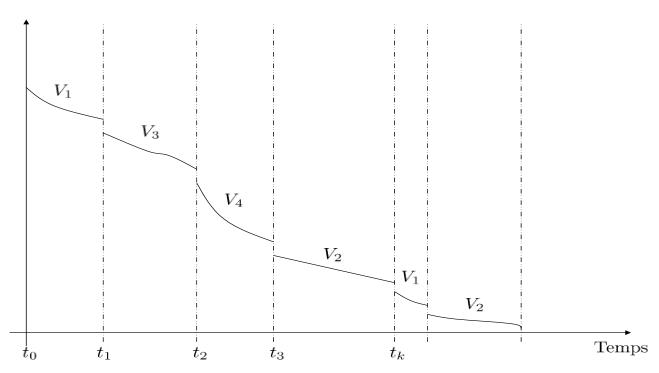
\includegraphics[scale=0.4]{images/decroissance.png}
	\caption{Évolution de la fonction d'énergie par morceaux}
	\label{fig:decroissance}
\end{figure}
%\pagebreak
\section{Le cas d'étude}
A présent, nous allons voir comment modéliser une mission de planification sur un cas concret, donc en intégrant le modèle d'un aéronef. Pour cela nous commencerons par présenter l'environnement et le modèle de l'aéronef. Ensuite nous décrirons les variables de notre problème, puis les contraintes.
\subsection{Le monde et l'aéronef}
La figure \ref{fig:scenarioVierge2} représente le monde et la mission (zones à éviter, point de départ et arrivée).
\begin{figure}[h]
	\centering	
	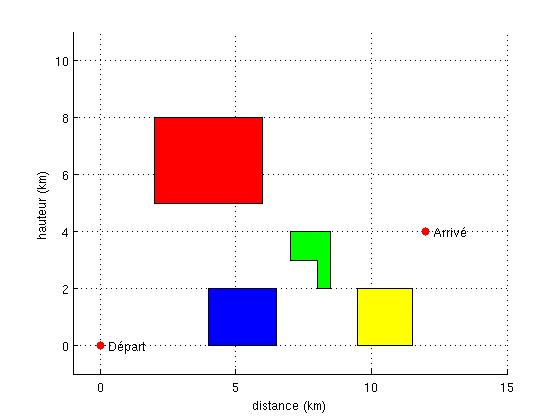
\includegraphics[scale=0.42]{images/scenarioVierge2.jpg}
	\caption{Environnement d'une mission}
	\label{fig:scenarioVierge2}
\end{figure}

L'aéronef que nous considérons pour cet exemple est celui sur lequel nous avons fait les tests lors de ce stage. Nous sommes partis d'un modèle non-linéaire (sous simulink) d'un avion de ligne présentant des changements de lois de pilotage autonome, et nous en avons extrait trois modèles linéaires (sous forme d'espace d'état Déf. \ref{defmodeleEtat}) représentant chaque mode de fonctionnement de façon séparée. Il est à noter que nous travaillons uniquement dans le plan longitudinal, donc la dynamique latérale n'est pas représentée dans ce modèle.
L'automate hybride résultant de cette manipulation est présenté sur la figure \ref{fig:modeleHybride}.
\begin{figure}[h]		
	\centering	
	\scalebox{0.8}{%
		\begin{tikzpicture}[->,>=stealth',shorten >=0pt,auto,node distance=0cm,
		semithick,every text node part/.style={align=center}]
		\tikzstyle{every state}=[fill=white,draw=black,text=black]

		%\node   (A)   at (2,1)  {};
		\node[state]    (maintien)  at (3,1.5)     {Maintien\\$-\epsilon < switch < \epsilon $};
		%\draw[<-] (B) to[bend right] (A)  ;
		
		\node[state]    (monter)   at (-2,-3.5)     {Montée\\$switch \geq \epsilon$ };
		\node[state]    (descendre)   at (8,-3.5)     {Descente\\$switch \leq -\epsilon$};
		
		\path 
		(maintien) edge [bend left=10]		node[below]{$switch \leq -\epsilon$}   (monter)		
		(maintien) edge [bend right=10] 	node[below]{$switch \geq \epsilon$}   (descendre)
		
		(monter) edge [bend left=10] 	node[left]{$switch < \epsilon$}   (maintien)		
		(monter) edge [bend left=10] 	node[above]{$switch \leq -\epsilon$}   (descendre)	
		
		(descendre) edge [bend left=10] 	node[below]{$switch \geq \epsilon$}  (monter)	
		(descendre) edge [bend right=10] 	node[right]{$switch > -\epsilon$}  (maintien)
		
		(maintien) edge [loop above]    	node[anchor=north,above]{} (maintien)	
		(monter) edge [loop below]    	node[anchor=south,below]{} (monter)
		(descendre) edge [loop below]    	node[anchor=south,below]{} (descendre);
		
		\end{tikzpicture} }
	\caption{Automate hybride autonome avec 3 lois de pilotage}
	\label{fig:modeleHybride}
\end{figure}

A chaque instant l'avion peut être dans un seul mode de fonctionnement, les changements de mode sont autonomes et se font en fonction de la valeur de $switch = |H_c - H|$, c'est à dire en fonction de la différence entre l'altitude de consigne et l'altitude réelle de l'avion.
Cette condition de switch et la valeur du $\epsilon$ sont imposées par le systèmes de l'avion.

A présent nous souhaitons savoir si cet aéronef est capable de remplir la mission donnée dans le monde décrit ci-dessus. La suite de ce chapitre va donc expliquer comment traduire cet exemple sous la forme d'un planificateur en CSP comme présenté dans la définition \ref{def:CSP-planif}.

\subsection{Les variables}
\label{subSec:variables}
Nous choisissons de distinguer trois différentes types de variables, les variables de \textbf{définition}, considérées comme constantes pour le planificateur. Les variables de \textbf{décision}, ce sont les variables sur lesquelles le planificateur a de la liberté. Enfin les variables de \textbf{fonction}, le planificateur ne peut pas directement fixer la valeur de ces variables, elles dépendent de variables de décision et de variable de définition. Cette distinction se retrouve dans certains outils de satisfaction de contraintes ou d'optimisation sous contraintes.
\pagebreak
\subsubsection{Les variables de définition}
\begin{itemize}		
	\item Les bornes du monde :
		\subitem $H_{max} \in \mathbb{R}^+$ : altitude maximale;
		\subitem $L_{max} \in \mathbb{R}^+$ : Longueur maximale; 
		\subitem $H_{min} \in \mathbb{R}^+$ : altitude minimale;
		\subitem $L_{min} \in \mathbb{R}^+$ : Longueur minimale; 
	\item Le point de départ :
		\subitem $H_{init} \in \mathbb{R}^+$ : altitude initiale;
		\subitem $L_{init} \in \mathbb{R}^+$ : distance initiale;
	\item Le point d'arrivé :
		\subitem $H_{goal} \in \mathbb{R}^+$ : altitude objectif;
		\subitem $L_{Goal} \in \mathbb{R}^+$ : distance objectif;
	\item L'aéronef :
		\subitem $Va_{min} \in \mathbb{R}^+$ : vitesse minimale;		\subitem $Va_{max} \in \mathbb{R}^+$ : vitesse maximale;
		\subitem $\alpha_{min} \in \mathbb{R}$ : angle d'incidence minimal;		\subitem $\alpha_{max} \in \mathbb{R}$ : angle d'incidence maximal;
	\item Autres :
	\subitem $step \in \mathbb{N}$ : le nombre d'itération, permet d'imposer au planificateur de tenter de résoudre le problème en un nombre d'itération fixé (lié au pas de temps);
	\subitem $t_{init} \in \mathbb{R}$ : l'instant initial du problème (en général $t(0) = 0$);
	\subitem $T_s \in \mathbb{R}^+$ : le pas de temps du système;
	\subitem $\epsilon \in \mathbb{R}^+$ : permet de définir la précision de l'objectif.
\end{itemize}	

\subsubsection{Les variables de décision}
\label{variableDecision}
Dans notre cas, nous souhaitons planifier la commande à appliquer à notre avion, cela revient à déterminer les valeurs du vecteur $U_k$ (Cf. éq \ref{eq:espaceEtat}). 

%Nous rappelons que notre planificateur doit travailler sur un horizon de temps borné à un nombre d'itération fixé. Chaque variable doit donc être calculée (et stockée) à chaque instant $k \in \{0, \ldots, step-1\}$.

Nous rappelons que notre planificateur doit travailler sur un horizon de temps borné à un nombre d'itérations fixé. Chaque variable doit donc être calculée (et stockée) à chaque instant $k \in \mathbb{N}^{step}$.

De plus, sur cet exemple nous n'avons que deux entrées :
\begin{itemize}	
	\item $\forall k, Vac_{k} \in \{Va_{min}, \ldots, Va_{max}\}$ : vitesse horizontale de consigne;	
	\item $\forall k, Hc_{k} \in \{H_{min}, \ldots, H_{max}\}$ : l'altitude de consigne.	
\end{itemize}

\subsubsection{Les variables de fonction}
\label{variableFonction}
Ce sont les variables les plus compliquées à définir, ce sont en général des fonctions mathématiques prenant en entrée plusieurs autres variables.

\underline{Les états du système} conditionnés par le mode de fonctionnement actuel ({$\mathbf{X_{k+1}}$}) :\\
\[\forall k, (mode_k == -1) \Rightarrow X_{k+1}(i) = \sum_{j=0}^{n-1} A_{descente}(i,j)\times X_k(j) + \sum_{j=0}^{m-1} B_{descente}(i,j)\times U_k(j)\]
\[\forall k, (mode_k == 0) \Rightarrow X_{k+1}(i) = \sum_{j=0}^{n-1} A_{maintien}(i,j)\times X_k(j) + \sum_{j=0}^{m-1} B_{maintien}(i,j)\times U_k(j)\]
\[\forall k, (mode_k == 1) \Rightarrow X_{k+1}(i) = \sum_{j=0}^{n-1} A_{mont\acute{e}}(i,j)\times X_k(j) + \sum_{j=0}^{m-1} B_{mont\acute{e}}(i,j)\times U_k(j)\]

\underline{Les 3 sorties du système} conditionnées par le mode de fonctionnement actuel ($\mathbf{Va_k, H_k}$ et $\mathbf{\alpha_k}$):\\
\[\forall k, (mode_k == -1) \Rightarrow 
	\left \{
	\begin{array}{l}
	Va_k = \sum_{j=0}^{n-1} C_{descente}(0,j)\times X_k(j) + \sum_{j=0}^{m-1} D_{descente}(0,j)\times U_k(j) \\
	H_k = \sum_{j=0}^{n-1} C_{descente}(1,j)\times X_k(j) + \sum_{j=0}^{m-1} D_{descente}(1,j)\times U_k(j) \\
	\alpha_k = \sum_{j=0}^{n-1} C_{descente}(2,j)\times X_k(j) + \sum_{j=0}^{m-1} D_{descente}(2,j)\times U_k(j)
	\end{array}
	\right.\]
	
	\[\forall k, (mode_k == 0) \Rightarrow 
	\left \{
	\begin{array}{l}
	Va_k = \sum_{j=0}^{n-1} C_{maintien}(0,j)\times X_k(j) + \sum_{j=0}^{m-1} D_{maintien}(0,j)\times U_k(j) \\
	H_k = \sum_{j=0}^{n-1} C_{maintien}(1,j)\times X_k(j) + \sum_{j=0}^{m-1} D_{maintien}(1,j)\times U_k(j) \\
	\alpha_k = \sum_{j=0}^{n-1} C_{maintien}(2,j)\times X_k(j) + \sum_{j=0}^{m-1} D_{maintien}(2,j)\times U_k(j)
	\end{array}
	\right.\]
	
	\[\forall k, (mode_k == 1) \Rightarrow 
	\left \{
	\begin{array}{l}
	Va_k = \sum_{j=0}^{n-1} C_{mont\acute{e}}(0,j)\times X_k(j) + \sum_{j=0}^{m-1} D_{mont\acute{e}}(0,j)\times U_k(j) \\
	H_k = \sum_{j=0}^{n-1} C_{mont\acute{e}}(1,j)\times X_k(j) + \sum_{j=0}^{m-1} D_{mont\acute{e}}(1,j)\times U_k(j) \\
	\alpha_k = \sum_{j=0}^{n-1} C_{mont\acute{e}}(2,j)\times X_k(j) + \sum_{j=0}^{m-1} D_{mont\acute{e}}(2,j)\times U_k(j)
	\end{array}
	\right.\]	
	
	\underline{Initialisation du mode} ($\mathbf{mode_0}$) :\\
	$(H_{goal} - H_{init}) \geq \epsilon \Rightarrow mode_0 = 1$ \\
	$(H_{goal} - H_{init}) \leq -\epsilon \Rightarrow mode_0 = -1$ \\
	$(\rceil((H_{goal} - H_{init}) \geq \epsilon) \wedge \rceil((H_{goal} - H_{init}) \leq -\epsilon) \geq \epsilon) \Rightarrow mode_0 = 0$ 
			
	\underline{La condition de switch} de l'automate hybride ($\mathbf{switch_k}$) :\\
	$\forall k, switch_k = Hc_k - H_k$
	
	\underline{La dynamique discrète} de l'automate ($\mathbf{mode_{k+1}}$):\\
	$\forall k < step, (mode_k == -1) \wedge (switch_k \geq \epsilon) \Rightarrow mode_{k+1} = 1$\\
	$\forall k < step, (mode_k == -1) \wedge (switch_k > -\epsilon) \Rightarrow mode_{k+1} = 0$ \\
	$\forall k < step, (mode_k == -1) \wedge (\rceil(switch_k \geq \epsilon) \wedge \rceil(switch_k > -\epsilon)) \Rightarrow mode_{k+1} = -1$\\ \\	
	$\forall k < step, (mode_k == 0) \wedge (switch_k \leq -\epsilon) \Rightarrow mode_{k+1} = 1$\\
	$\forall k < step, (mode_k == 0) \wedge (switch_k \geq \epsilon) \Rightarrow mode_{k+1} = -1$ \\
	$\forall k < step, (mode_k == 0) \wedge (\rceil(switch_k \leq -\epsilon) \wedge \rceil(switch_k \geq \epsilon)) \Rightarrow mode_{k+1} = 0$\\ \\	
	$\forall k < step, (mode_k == 1) \wedge (switch_k < \epsilon) \Rightarrow mode_{k+1} = 0$\\
	$\forall k < step, (mode_k == 1) \wedge (switch_k \leq -\epsilon) \Rightarrow mode_{k+1} = -1$ \\
	$\forall k < step, (mode_k == 1) \wedge (\rceil(switch_k < \epsilon) \wedge \rceil(switch_k \leq -\epsilon)) \Rightarrow mode_{k+1} = 1$
			
	\underline{Le temps} ($\mathbf{t_k}$) :\\
	$\forall k, t_k = t_{init} + T_s\times k$
	
	\underline{La distance parcourue} ($\mathbf{L_k}$) :\\
	$\forall k, L_k = L_{init} + Va_k\times T_s$
	
	\underline{La fonction de coût}, il s'agira ici de minimiser l'écart entre l'altitude objectif et l'altitude réelle au dernier instant de temps :\\
	$but = |H_{step-1} - H_{goal}|$
	


\subsection{Les contraintes}
A l'aide des variables décrites précédemment nous pouvons définir les contraintes CSP permettant au solveur de prendre en compte les obstacles, les bornes du monde etc...

	\underline{Le monde} : \\
	$\forall k, Va_{min} \leq Va_k \leq Va_{max}$ : contrainte sur la vitesse réelle.\\
	$\forall k, H_{min} \leq H_k \leq H_{max}$ : contrainte sur l'altitude réelle.\\
	$\forall k, \alpha_{min} \leq \alpha_k \leq \alpha_{max}$ : contrainte sur l'angle d'incidence réel.\\
	$\forall k, L_{min} \leq L_k \leq L_{max}$ : permet de connaitre la position en distance de l'avion.\\	
	\underline{Les obstacles} : \\
	Nous allons détailler ici les 4 zones présentées sur la figure \ref{fig:scenarioVierge2}. \\
	zone rouge : $\forall k, 2 \leq L_k \leq 6 \Rightarrow H_k > 8 \vee H_k < 5$\\
	zone bleue : $\forall k, 4 \leq L_k \leq 6.5 \Rightarrow H_k > 2$\\
	zone verte : $\forall k,   \left \{
	\begin{array}{l}
	7 \leq L_k < 8.5 \Rightarrow H_k > 4 \vee H_k < 3 \\
	8.5 \leq L_k \leq 9 \Rightarrow H_k > 4 \vee H_k < 2
	\end{array}
	\right.$\\
	zone jaune : $\forall k, 9.5 \leq L_k \leq 11.5 \Rightarrow H_k > 2$\\
	\underline{La mission} : \\
	$H_{0} == H_{init}$ : permet d'imposer l'altitude initiale.\\
	$L_{0} == L_{init}$ : permet d'imposer la distance initiale.\\
	$H_{goal} - \epsilon \leq H_{step} \leq H_{goal} + \epsilon$ : permet de définir une altitude à atteindre avec une incertitude de précision\\
	$l_{goal} - \epsilon \leq L_{step} \leq L_{goal} + \epsilon$ : permet de définir une distance à atteindre avec une incertitude de précision\\
	\underline{La stabilité} :\\
	Pour rappel, nous souhaitons que l'aéronef reste dans son domaine de stabilité à chaque instant, et ce, même lors d'un changement de mode. Pour cela nous reprenons les résultats présentés dans la partie \ref{subsubsec:stabHybride}, c'est à dire qu'à chaque changement de mode, la valeur de la fonction $V(x) = x^TPx$ doit diminuer.
	
	 %Pour cela nous proposons qu'à chaque instant, le système (donc le vecteur $x_k$) respecte les contraintes ellipsoïdales décrites dans le paragraphe \ref{subsection:contrainteStabilite}. De plus lors d'un changement de mode, nous souhaitons que $x_k$ soit dans l'intersection des ellipsoïdes des 2 modes en question.
	
	Pour faciliter l'écriture des contraintes, nous introduisons les notations suivantes : 
%	\vspace{-1cm}
	\begin{tabbing}
		\hspace{5cm}\=\hspace{5cm}\=\kill
	$\mathcal{V}_{-1,k} = x_k^TP_{descente}x_k$	\> $\mathcal{V}_{0,k} = x_k^TP_{maintien}x_k$ \> $\mathcal{V}_{1,k} = x_k^TP_{mont\acute{e}e}x_k$
	\end{tabbing} 
%	\begin{itemize}
%		\centering
%		\item[ ] $\mathcal{V}_{-1,k} = x_k^TP_{descente}x_k$;
%		\item[ ] $\mathcal{V}_{0,k} = x_k^TP_{maintien}x_k$;
%		\item[ ] $\mathcal{V}_{1,k} = x_k^TP_{mont\acute{e}e}x_k$;
%		%\item[ ] $\mathcal{E}_{-1,k}$ représente l'ellipsoïde du mode descente à l'instant k : $x_k^TP_{descente}x_k < 1$;
%		%\item[ ] $\mathcal{E}_{0,k} \equiv x_k^TP_{descente}x_k < 1$;		%\item[ ] $\mathcal{E}_{1,k} \equiv x_k^TP_{mont\acute{e}}x_k < 1$.
%	\end{itemize}
	
%	Les contraintes sont donc les suivantes :
%	$\forall k, (mode_k == 0) \wedge (mode_{k+1} == 0) => \mathcal{E}_{0,k} \wedge \mathcal{E}_{0,k+1}$\\
%	$\forall k, (mode_k == 0) \wedge (mode_{k+1} == -1) => \mathcal{E}_{0,k} \wedge \mathcal{E}_{-1,k} \wedge \mathcal{E}_{0,k+1} \wedge \mathcal{E}_{-1,k+1}$\\
%	$\forall k, (mode_k == 0) \wedge (mode_{k+1} == 1) => \mathcal{E}_{0,k} \wedge \mathcal{E}_{1,k} \wedge \mathcal{E}_{0,k+1} \wedge \mathcal{E}_{1,k+1}$\\\\
%	$\forall k, (mode_k == -1) \wedge (mode_{k+1} == -1) => \mathcal{E}_{-1,k} \wedge \mathcal{E}_{-1,k+1}$\\
%	$\forall k, (mode_k == -1) \wedge (mode_{k+1} == 0) => \mathcal{E}_{-1,k} \wedge \mathcal{E}_{0,k} \wedge \mathcal{E}_{-1,k+1} \wedge \mathcal{E}_{0,k+1}$\\
%	$\forall k, (mode_k == -1) \wedge (mode_{k+1} == 1) => \mathcal{E}_{-1,k} \wedge \mathcal{E}_{1,k} \wedge \mathcal{E}_{-1,k+1} \wedge \mathcal{E}_{1,k+1}$\\\\
%	$\forall k, (mode_k == 1) \wedge (mode_{k+1} == 1) => \mathcal{E}_{1,k} \wedge \mathcal{E}_{1,k+1}$\\
%	$\forall k, (mode_k == 1) \wedge (mode_{k+1} == -1) => \mathcal{E}_{1,k} \wedge \mathcal{E}_{-1,k} \wedge \mathcal{E}_{1,k+1} \wedge \mathcal{E}_{-1,k+1}$\\
%	$\forall k, (mode_k == 1) \wedge (mode_{k+1} == 0) => \mathcal{E}_{1,k} \wedge \mathcal{E}_{0,k} \wedge \mathcal{E}_{1,k+1} \wedge \mathcal{E}_{0,k+1}$\\\\
Les contraintes sont donc les suivantes :
\begin{center}
$
\begin{array}{lcl}
\forall k, (mode_k == 0) \wedge (mode_{k+1} == 0)	& => & \mathcal{V}_{0,k+1} \leq \mathcal{V}_{0,k} \\ 
\forall k, (mode_k == 0) \wedge (mode_{k+1} == -1)	& => & \mathcal{V}_{-1,k+1} \leq \mathcal{V}_{0,k} \\ 
\forall k, (mode_k == 0) \wedge (mode_{k+1} == 1)	& => & \mathcal{V}_{1,k+1} \leq \mathcal{V}_{0,k} \\ \\

\forall k, (mode_k == -1) \wedge (mode_{k+1} == -1)	& => & \mathcal{V}_{-1,k+1} \leq \mathcal{V}_{-1,k} \\ 
\forall k, (mode_k == -1) \wedge (mode_{k+1} == 0)	& => & \mathcal{V}_{0,k+1} \leq \mathcal{V}_{-1,k} \\ 
\forall k, (mode_k == -1) \wedge (mode_{k+1} == 1)	& => & \mathcal{V}_{1,k+1} \leq \mathcal{V}_{-1,k} \\ \\

\forall k, (mode_k == 1) \wedge (mode_{k+1} == 1)	& => & \mathcal{V}_{1,k+1} \leq \mathcal{V}_{1,k} \\ 
\forall k, (mode_k == 1) \wedge (mode_{k+1} == -1)	& => & \mathcal{V}_{-1,k+1} \leq \mathcal{V}_{1,k} \\ 
\forall k, (mode_k == 1) \wedge (mode_{k+1} == 0)	& => & \mathcal{V}_{0,k+1} \leq \mathcal{V}_{1,k} \\ 
\end{array} 
$
\end{center}
%		$\forall k, (mode_k == 0) \wedge (mode_{k+1} == 0) => \mathcal{V}_{0,k+1} \leq \mathcal{V}_{0,k}$\\
%		$\forall k, (mode_k == 0) \wedge (mode_{k+1} == -1) => \mathcal{V}_{-1,k+1} \leq \mathcal{V}_{0,k}$\\
%		$\forall k, (mode_k == 0) \wedge (mode_{k+1} == 1) => \mathcal{V}_{1,k+1} \leq \mathcal{V}_{0,k}$\\\\
%		$\forall k, (mode_k == -1) \wedge (mode_{k+1} == -1) => \mathcal{V}_{-1,k+1} \leq \mathcal{V}_{-1,k}$\\
%		$\forall k, (mode_k == -1) \wedge (mode_{k+1} == 0) => \mathcal{V}_{0,k+1} \leq \mathcal{V}_{-1,k}$\\
%		$\forall k, (mode_k == -1) \wedge (mode_{k+1} == 1) => \mathcal{V}_{1,k+1} \leq \mathcal{V}_{-1,k}$\\\\
%		$\forall k, (mode_k == 1) \wedge (mode_{k+1} == 1) => \mathcal{V}_{1,k+1} \leq \mathcal{V}_{1,k}$\\
%		$\forall k, (mode_k == 1) \wedge (mode_{k+1} == -1) => \mathcal{V}_{-1,k+1} \leq \mathcal{V}_{1,k}$\\
%		$\forall k, (mode_k == 1) \wedge (mode_{k+1} == 0) => \mathcal{V}_{0,k+1} \leq \mathcal{V}_{1,k}$\\\\
	\noindent
	\shadowbox{\begin{minipage}{\textwidth}
			\textbf{Résumé :} Dans ce chapitre nous avons présenté un problème de planification dans un formalisme de CSP.
			
			Une description mathématique de la modélisation de l'environnement, de la mission et de l'aéronef a été effectuée, cette modélisation se veut assez généraliste dans le but de pouvoir l'appliquer à différentes mission et différents aéronefs.
			
			Enfin un modèle a été détaillé qui ne s'appuie pas sur un solveur CSP en particulier, la suite de ce rapport décrit l'implémentation de ce problème sur différents solveurs.	
		\end{minipage}}
	

